\chapter{Introduction}
\pagenumbering{arabic} 
\setcounter{page}{1} 

Despite more than a century of active biology research, many biological systems lack good computational models.
Computational models are only useful if they accurately represent how the underlying biological system behaves.
When these models are faithful to the underlying biology, experiments can be run \textit{in silico} instead of \textit{in vivo}, speeding up the pace of research.
%A good model should also be consistent---running it multiple times should produce the same results.
%Though biological experiments can have wide variance due to external conditions, we want our model to vary only due to intrinsic biological sources of variation.
%Exact reproducibility is very difficult in laboratory environments, but a computer model can and should eliminate the extrinsic sources of variance that one encounters in a laboratory setting.
The best computational models are useful not only as biology simulators, but also as facilitators of new hypotheses.
Computational biology models should both help researchers improve their understanding of the modeled system and surface novel insights into the underlying biology.

%TODO: maybe remove?
%Recent efforts to model biological systems have become ever more accurate as the amount of biological data collected increases.
Biological systems are complex and can be examined at many different levels.
For example, one model could use a physical description of a cell to predict its shape as it grows.
A different model could use -omic data---genomic, transcriptomic, and metabolomic measurements---to model the production of compounds that allow for cellular growth.
We will focus on modeling the metabolism of a biological system.
%As all models are inherently limited in some way, so the choice of the type of model that is used to describe a system is extremely important.

The goal of this dissertation is to provide a model for biologists to better understand what is occurring in cell-free systems.
This dissertation details an end-to-end system that produces metabolic models for cell-free systems based on experimental data.
Our system learns which reactions are most important for a given cell-free system and produce a reduced metabolic model that fits with the experimental data.
We utilize a Variational Autoencoder (\gls{vae}) on top of a common metabolic modeling technique called Flux Balance Analysis (\gls{fba}) to produce these reduced models.
In particular, we introduce a new loss function for the \gls{vae} that allows us to effectively reduce the dimensionality of the model based on our experimental data.
We hope that our system will be used by biologists to better understand how different starting conditions might affect their experiments, cope with batch variation, and gain a deeper understand of the composition of cell-free systems.

\textbf{Metabolic models}

%TODO: fix this paragraph--why is it relevant/here?
Metabolism is defined as all of the chemical reactions that occur within an entity---usually an organism or a cell---in order to sustain its life and growth.
Biologists are interested in how the metabolism of a system works as it is the end result of the other biological process of interest (e.g. transcription and translation).
While ongoing work continues to develop a more robust understanding of metabolism, recent advances have begun to explore applications that involve engineering the metabolism. 
Metabolic engineering has the potential to create novel advances in medicine and energy production~\cite{keasling2012synthetic}.
Metabolic models are an important tools for metabolic engineers because they can be used to predict how the phenotype of an organism will respond to attempts to engineer it.

%TODO: fix this sentence
Most metabolic models represent the chemical reactions in a cell with a mathematical representation of the reaction coefficients.
Individual reactions are denoted as equations in these models.
Mathematical constraints are placed on these reactions based on our knowledge of biological pathways.
Models of this type are collected under the heading of \gls{cobra} models~\cite{schellenberger2011quantitative} and are very common among the metabolic engineering community~\cite{orth2010flux}.
\gls{fba} is one of the most popular metabolic modeling techniques.
It has been used in hundreds of different works to model metabolism~\cite{feist2008growing}.
These applications range from optimizing metabolic pathways~\cite{almaas2004global} to investigating gene networks~\cite{shlomi2007genome}.
\gls{fba} is based on a genome-scale metabolic models (\glspl{gem}) reconstructed from the genome of an organism of interest.
However, these \glspl{gem} describe living organisms, not cell-free systems, so typical \gls{fba} models cannot be applied out of the box to a cell-free system.

\textbf{Cell-free systems}

Cell-free Protein Synthesis (\gls{cfps}) systems are a reduced version of cells that allows these systems to produce proteins without being alive.
The Central Dogma of biology, as enunciated by Francis Crick, is that \gls{dna} makes \gls{rna} makes protein~\cite{crick1970central}.
While this may be a slight oversimplification, the key idea is that the production of proteins is the end goal for most biological systems.
\gls{cfps} systems take that to an extreme by removing all endogenous \gls{dna}, \gls{rna}, and membranes while retaining the machinery for transcription and translation.

A \gls{cfps} system is therefore a type of programmable matter, a veritable biological computer.
The \gls{cfps} system acts like a computer because it can "execute" any \gls{dna} "program" that is added to the mixture.
The output of a \gls{cfps} system is determined by which \gls{dna} program is loaded into a cell-free system.
This simplicity has made cell-free systems popular for a wide array of applications~\cite{hodgman2012cell, rollin2013new, carlson2012cell}.
Additionally, cell-free systems have been shown to be extremely cheap, costing less than \$0.01 per \gls{ul} of reaction~\cite{murray2013cost}.

\gls{cfps} systems have two key aspects that make it an ideal platform to model for this dissertation.
First of all, running experiments in a \gls{cfps} system is much faster than typical \textit{in vivo} methods because performing an experiment does not require growing cells.
This meant that we were able to start from scratch and generate relevant data within several weeks instead of the many months or years that a cell-based system could take.
\gls{cfps} systems are also simpler than a full cellular system, and should therefore be easier to model accurately.
By definition, \gls{cfps} systems contain a strict subset of the reactions that occur in a cell-based system.
The key issue is that we do not know which reactions are included in that subset.

Despite their reduced nature, \gls{cfps} systems lack good models.
Modeling \gls{cfps} systems is difficult because \gls{cfps} systems are composed of blended cells and therefore we do not know exactly what is in the system.
However, few prior attempts at modeling \gls{cfps} systems have used metabolic models to examine \gls{cfps} systems.
We believe that metabolic models are a natural fit to model \gls{cfps} systems.
Since \gls{cfps} are not living organisms, their effectiveness is entirely based on reaction constraints and energy regeneration.
Thus, understanding the metabolism of these systems is extremely important.
The few existing metabolic models for \gls{cfps} systems have been hand-constructed by a specific lab~\cite{bujara2012silico, vilkhovoy2017sequence}.
We provide an automated system to reduce standard \glspl{gem} to metabolic models of \gls{cfps} systems.

%TODO add contributions
\textbf{Contributions}

This dissertation makes a number of contributions in the field of metabolic modeling and dimensionality reduction for \gls{cfps} systems.
\begin{itemize}
\item We provide one of the first applications of deep learning to metabolic models.
We show that using a \gls{vae} is more effective than \gls{pca} with regards to building a reduced metabolic model.
Since \gls{pca} is a common dimensionality reduction technique in biology, this motivates other work applying \glspl{vae} instead of \gls{pca}..
\item We also introduce a new loss function for \glspl{vae} that incorporates a correlation loss term.
Although we focused specifically on using it for experimental data generated from \gls{cfps} systems, the loss function is general and could be used in any application with experimental data.
\item Finally, we produce a number of new, reduced models for \gls{cfps} systems.
These models can be used by biologists and metabolic engineers working with these \gls{cfps} systems.
%\item Finally, we uncovered a number of biological insights
%\item This dissertation provides an end-to-end system to generate models for \gls{cfps} systems.
%Given biological data generated in a lab, the computational pipeline will then produce a metabolic model for the given \gls{cfps} system.
%\item Within that framework, we provide a the first automated reduction system that tailors \glspl{gem} specifically for \gls{cfps} systems.
%That means our system can be used for any cell-free system that is derived from an organism that has a fully specified GEM, of which there are many dozens.
%\item Additionally, this is one of the first applications of deep learning or autoencoders to \gls{fba} models.
%As deep learning becomes ever more popular, our system provide an early example of how it may be incorporated into the field of metabolic modeling.
\end{itemize}
%VAE
%experiments + computational
%latent representation
We note that our approach was designed to be as general as possible, which has two key benefits.
Our system can be applied out-of-the-box to other types of cell-free systems; i.e. systems that use cells from organisms other than \gls{ecoli}.
Additionally, the techniques developed here for modeling cell-free systems can be applied to modeling any biological system that uses experimental data and metabolic models.

\textbf{Outline}
\begin{figure}[t!]
\begin{center}
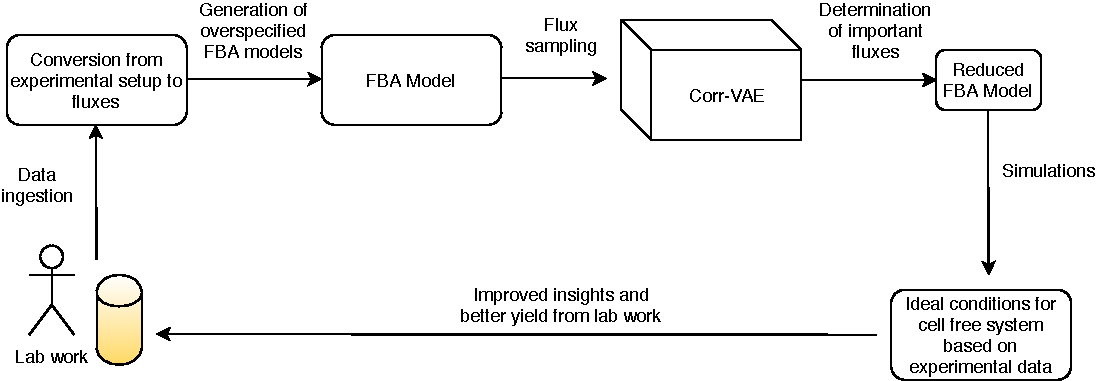
\includegraphics[width=\textwidth]{figs/SystemOverview.pdf}
\end{center}
\label{fig:overview}
\caption{A figure showing the overall pipeline for the system to generate cell-free metabolic models.}
\end{figure}

The structure of this dissertation is as follows.
%TODO add back in?
Chapter \ref{chap:bkg} provides background information on cell-free systems, \gls{fba}, and \glspl{vae}.
%We describe the different types of cell-free systems, how we produce our system, and some uses and advantages for cell-free systems.
%Then, we explore the mathematical foundations of \gls{fba} and how it can be used to model biological systems.
%Finally, we explain how autoencoders are used for dimensionality reduction, specifically focusing on how VAEs work.
Chapter \ref{chap:rw} provides related work in the fields of metabolic models, reduction of metabolic models, modeling cell-free systems, and \glspl{vae}.
%We analyze the current state of the art in metabolic modeling, specifically focusing on the development of \gls{fba} and the creation of a GEM for \ecoli.
%Next, we focus on how search techniques have been used to reduce metabolic models to their core reactions.
%Then, we share efforts to model cell-free systems, describing two prior works that have applied \gls{fba} to cell-free systems.
%Finally, we outline the relevant literature about VAEs.
Chapter \ref{chap:impl} describes the system we have designed and built to model cell-free systems (shown in Figure \ref{fig:overview}).
%We begin by describing our experimental setup and how we generated our data.
%Next, we detail how to ingest the experimental setup and data and convert it into a metabolic model.
%Then, we explain how we used that model to generate a larger dataset for our deep learning algorithms.
%Lastly, we use that dataset to train a VAE, which generates a lower dimensionality representation that can be used to create better cell-free metabolic models.
Chapter \ref{chap:res} describes the results of using a \gls{vae} to reduce \gls{fba} models.
Notably, we show that our reduced models are better at describing \gls{cfps} systems than both \glspl{gem} and already published reduced models.
%We also show novel biological insights that were unearthed due to my system.
%Finally, we illustrate how a model can be learned on one set of biological data and transfer to a different set of data. 
We conclude with a discussion of future work in this area.
